\documentclass[12pt]{article}

\usepackage{qtree}
\usepackage{tikz}

\begin{document}

\section{Using qtree}

\Tree [.S a [.NP {\bf b} c ] d ]

\subsection{Intro tree 1}

\Tree [.+ 5 [.* 2 3 ] ]

\subsection{Intro tree 2}

\Tree [.* [.+ 5 2 ] 3 ]

\section{Using tikz}

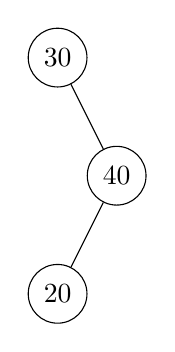
\begin{tikzpicture}
\node[circle,draw](z){$30$}
  child[missing]{}
  child{
    node[circle,draw]{40} child{node[circle,draw] {20}} child[missing] };
\end{tikzpicture}

\subsection{Intro tree 1}

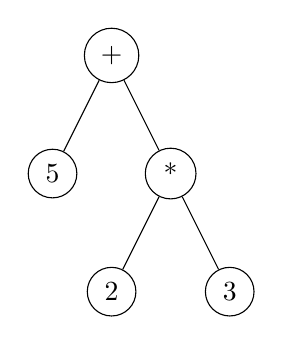
\begin{tikzpicture}
  \node[circle,draw](z){+}
    child{
        node[circle,draw]{5}
    }
    child{
        node[circle,draw]{*}
            child{node[circle,draw]{2}}
            child{node[circle,draw]{3}}
    };
\end{tikzpicture}

\subsection{Intro tree 2}

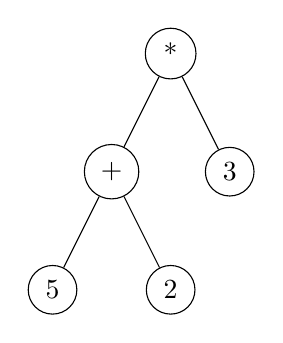
\begin{tikzpicture}
  \node[circle,draw](z){*}
    child{
        node[circle,draw]{+}
            child{node[circle,draw]{5}}
            child{node[circle,draw]{2}}
    }
    child{
        node[circle,draw]{3}
    }
    ;
\end{tikzpicture}

\subsection{Intro tree 2}

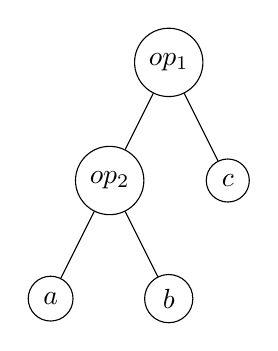
\begin{tikzpicture}
  \node[circle,draw](z){$op_1$}
    child{
        node[circle,draw]{$op_2$}
            child{node[circle,draw]{$a$}}
            child{node[circle,draw]{$b$}}
    }
    child{
        node[circle,draw]{$c$}
    }
    ;
\end{tikzpicture}

\subsection{Intro tree 1}

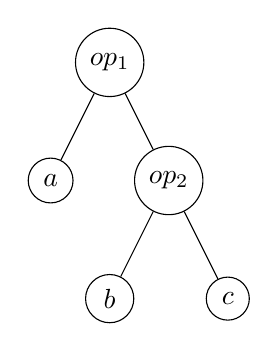
\begin{tikzpicture}
  \node[circle,draw](z){$op_1$}
    child{node[circle,draw]{$a$}}
    child{
        node[circle,draw]{$op_2$}
            child{node[circle,draw]{$b$}}
            child{node[circle,draw]{$c$}}
    }
    ;
\end{tikzpicture}

\subsection{Intro tree 2}

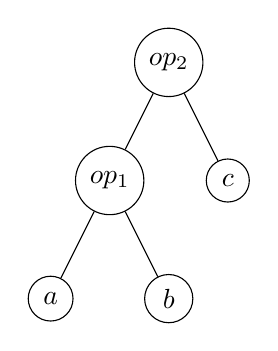
\begin{tikzpicture}
  \node[circle,draw](z){$op_2$}
    child{
        node[circle,draw]{$op_1$}
            child{node[circle,draw]{$a$}}
            child{node[circle,draw]{$b$}}
    }
    child{
        node[circle,draw]{$c$}
    }
    ;
\end{tikzpicture}

\end{document}